\section{byte codes}

The FLIP-8 CPU works with simple 8 bit instructions. The different compute modes (Immediate, Compute, Copy and Condition) are separated with the two most significant bits. The rest of the instructions are in the remaining six bits.

\subsection{Overview}

\begin{figure}[ht]
    \center
    \begin{bytefield}[bitwidth=40pt,bitheight=20pt]{8}
        \bitheader{0-7} \\
        \bitbox{2}{Mode} &
        \bitbox{6}{Opcode}
    \end{bytefield}
    \caption{instruction structure}
\end{figure}

\begin{table}[ht]
    \center
    \begin{tabular}{c|l}
    Byte representation & Mode \\ \hline
    \drawbits{0,0,X,X,X,X,X,X} & Immediate \\
    \drawbits{0,1,X,X,X,X,X,X} & Compute \\
    \drawbits{1,0,X,X,X,X,X,X} & Copy \\
    \drawbits{1,1,X,X,X,X,X,X} & Condition
\end{tabular}
    \caption{Main CPU Modes}
\end{table}


\subsubsection{Immediate Mode}

When the CPU is in Immediate Mode the programmer is able to inject values in the first registry.
With the remaining six bits the can use up to 64 numbers. These could be used for custom flags.

\begin{figure}[ht]
    \center
    \begin{bytefield}[bitwidth=40pt,bitheight=20pt]{8}
        \bitheader{0-7} \\
        \bitbox{2}{Immediate} &
        \bitbox{6}{Number}
    \end{bytefield}
    \caption{immediate mode}
\end{figure}

\begin{figure}[ht]
    \center 
    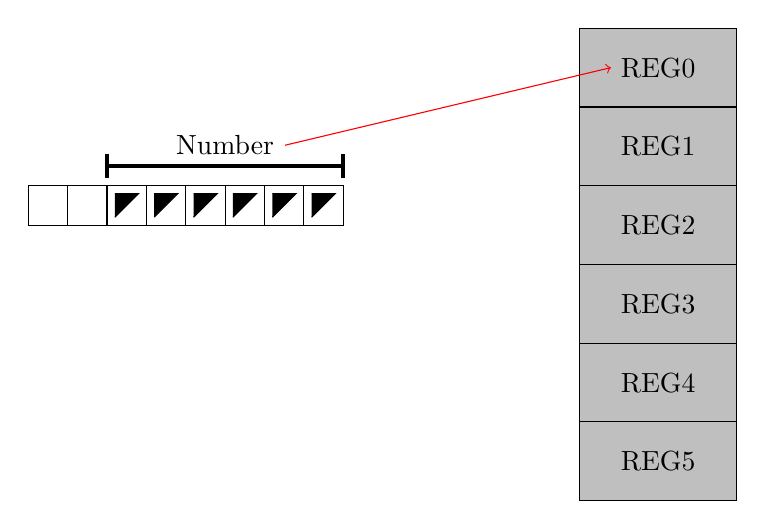
\begin{tikzpicture}
    \filldraw[fill=lightgray] (0,0) rectangle (2,1) node[pos=.5] {REG5};
    \filldraw[fill=lightgray] (0,1) rectangle (2,2) node[pos=.5] {REG4};
    \filldraw[fill=lightgray] (0,2) rectangle (2,3) node[pos=.5] {REG3};
    \filldraw[fill=lightgray] (0,3) rectangle (2,4) node[pos=.5] {REG2};
    \filldraw[fill=lightgray] (0,4) rectangle (2,5) node[pos=.5] {REG1};
    \filldraw[fill=lightgray] (0,5) rectangle (2,6) node[pos=.5] (reg0) {REG0};

    \foreach \x in {-7,-6.5,...,-6}{
        \draw (\x,4) rectangle (\x+0.5,3.5);
    }
        
    \foreach \x in {-6,-5.5,...,-3.5}{
        \draw (\x,4) rectangle (\x+0.5,3.5);
        \filldraw[fill=black] (\x+0.1,3.9) -- (\x+0.4,3.9) -- (\x+0.1,3.6);
    }

    \draw [line width=0.5mm](-6,4.4) -- (-6,4.1);
    \draw [line width=0.5mm](-3,4.4) -- (-3,4.1);
    \draw [line width=0.5mm](-6,4.25) -- (-3,4.25) node[pos=.5, above] (N) {Number};

    \draw [->,red] (N.east) to (reg0.west);
\end{tikzpicture}
    \caption{Immediate Mode Register}
\end{figure}

\newpage
\subsubsection{Compute}

When the CPU is in Compute Mode the ALU uses the two numbers in REG1 and REG2 and stores the output of the selected Operation in REG3. The Operations can be selected with the opcode. The available Operation can be found in \autoref{fig:Compute}.

\begin{table}[ht]
    \center
    \begin{tabular}{c|l}
    Opcode & ALU Mode \\ \hline
    \drawbits{0,1,0,0,0,0,0,0} & OR \\
    \drawbits{0,1,0,0,0,0,0,1} & NAND \\
    \drawbits{0,1,0,0,0,0,1,0} & NOR \\
    \drawbits{0,1,0,0,0,0,1,1} & AND \\
    \drawbits{0,1,0,0,0,1,0,0} & ADD \\
    \drawbits{0,1,0,0,0,1,0,1} & MINUS
\end{tabular}
    \caption{Compute Operation}
    \label{fig:Compute}
\end{table}